\section{简介:结构、流程与次序}
\subsection*{编译器如何处理代码?}
在2.3节中,我们提到过``语法''和``语义''的区别。语法正确与否,事关代码能否通过编译;而语义正确与否,则事关程序能否实现我们想要的功能。在编译期,预处理器会进行一系列预处理,例如把 \lstinline@iostream@ 头文件的内容复制到我们的代码中,以便编译器进行编译。有些值也是在编译期进行计算的,比如 \lstinline@sizeof@。这类处理和计算过程早在编译结束之前就已经操作完毕,我们将其统称为\textbf{编译时行为(Compile-time behaviour)}。\par
\begin{lstlisting}
    int a {3};
    cout << sizeof a << endl; //输出a的内存占用
    cout << sizeof (double); //输出double的内存占用
\end{lstlisting}
之所以这种操作在编译时就可以算出来,是因为编译器在编译期就已经可以确定它的值。还记得吗,无论 \lstinline@a@ 的值如何变化,它占用的内存空间总是那些,不会变多和变少。换言之,无论 \lstinline@a@ 的值是多少,\lstinline@sizeof a@ 总是一个在编译时就可以确定下来的常量。那么在编译时就把它计算出来,当然更划算了。\par
另一些操作,我们在编译时不能确定它的值,所以需要在程序运行时,具体情况具体分析。比如 \lstinline@x+y@(假如 \lstinline@x@ 和 \lstinline@y@ 是两个变量),这个运算结果当然依赖于具体变量的值,无法预测,所以要在编译时求解。我们将其统称为\textbf{运行时行为(Runtime behaviour)}。以下所列代码均为运行时行为。
\begin{lstlisting}
    double d; //定义double型变量d,程序为其分配内存空间
    cin>>d; //输入d的值
    d=d*d; //为d赋值
    cout<<d; //输出d的值
\end{lstlisting}\par
读者可能好奇,代码1.2中的操作有哪些是编译时行为,哪些是运行时行为呢?事实上,只有 \lstinline@include@ 和 \lstinline@using@ 语句是编译时行为;而 \lstinline@double@ 变量的定义、表达式的计算和输出,全部是运行时行为。\par
编译器没有人那么智能。它判断这个表达式能否在编译时操作的依据是``它是否在编译时就能确定下来''。由变量构成的表达式当然不满足这样的条件(因为变量可以在任何时候发生改变),于是编译器一刀切,认为只要有变量参与,这个表达式就不能在编译期求得。\par
那么常量呢?看似可以,但它也不总是可行的!我们在2.1节中介绍过,常量是可以用变量来初始化的。
\begin{lstlisting}
    int g; //定义一个临时变量g
    cin >> g; //通过输入来改变g的值
    const int Grid = {g}; //用g的值来为常量Grid初始化
\end{lstlisting}
也就是说,常量的值也未必能在编译期就确定下来。一般来说,编译器会对实际情况进行判断,如果一个常量能在编译期求出,这就是编译时行为;否则就放在运行期求出,这是运行时行为。\par
另外就是,字面量构成的表达式也可以在编译期求得。比如说
\begin{lstlisting}
    int a {15+8/2-3}; //定义变量a并初始化为14
\end{lstlisting}
请注意,``\lstinline@15+8/2-3@ 的计算''和``定义数据并初始化''是两个过程!计算过程中只涉及字面量,所以编译器可以直接求得,这是编译时行为;而变量的定义和初始化是无法在编译期就完成的,这是运行时行为。\par
C++11以后的标准允许我们定义\textbf{常量表达式(Constant expression)},来拓展编译时行为的可能性。我们可以把它理解成一种新型的字面量\footnote{事实上,常量表达式是字面量的超集。但用字面量的思路来理解常量表达式要容易得多。}。
\begin{lstlisting}
    constexpr double Pi {3.14159}; //定义常量表达式Pi,现在Pi是一个字面量啦
    constexpr double Pi2 {Pi * Pi}; //定义常量表达式Pi2,现在Pi2也是一个字面量
\end{lstlisting}
仅由字面量(广义地说,常量表达式)构成的表达式可以在编译期求出,比如这里的 \lstinline@Pi*Pi@。但假如中间环节出现了变量,或者是不能在编译时确定下来的常量,那么就会出现问题。
\begin{lstlisting}
    const double Pi {3.14159}; //定义常量Pi,它不是常量表达式,不能视为字面量
    constexpr double Pi2 {Pi * Pi}; //试图用Pi来定义常量表达式Pi2
//error: the value of 'Pi' is not usable in a constant expression
\end{lstlisting}
编译器报错,显示信息为``\lstinline@Pi@ 的值不能用于常量表达式中''。这说明我们必须用常量表达式构成的表达式来定义常量表达式。\par
我们此前介绍过 \lstinline@numeric_limits<int>::max()@ 这类的写法,它也是常量表达式。编译器能够直接算出这个值,并把它当作字面量来看待,就不需要运行时再去计算了。\par
\subsection*{控制台如何处理输入/输出}
源代码经过编译和链接等步骤形成的文件多种多样。有些是库文件(Library),它们可以作为目标文件(Object file)与其它文件链接,我们暂不讨论;有些是可执行文件(Executable),我们在前两章中有三个完整的\texttt{.cpp}代码,可以编译成可执行文件(如果你使用Windows,那么这类文件的扩展名就是\texttt{.exe}),并给我们输出执行结果。当然还有其它的形式,比如多媒体,我就不一一列举了。\par
可执行文件也多种多样。有些是图形用户界面(Graphical user interface, GUI)的,有些是文本用户界面(Text-based user interface, TUI),还有些则是命令行界面(Command-line interface, CLI)的。\par
早期的电脑为用户提供的都是命令行界面,用户和电脑之间通过纯文本来进行交互。这种方式不直观,也很难用,用户通过键盘来输入纯文本,电脑通过显示器来输出纯文本。这就给计算机学习造成很高的门槛。\par
文本用户界面主要基于文本,但相比命令行界面来说,在操作上要轻松一些。用户可以使用鼠标和键盘来控制输入。图3.1是一个基于文本用户界面的控制台程序。\par
\begin{figure}[htbp]
    \centering
    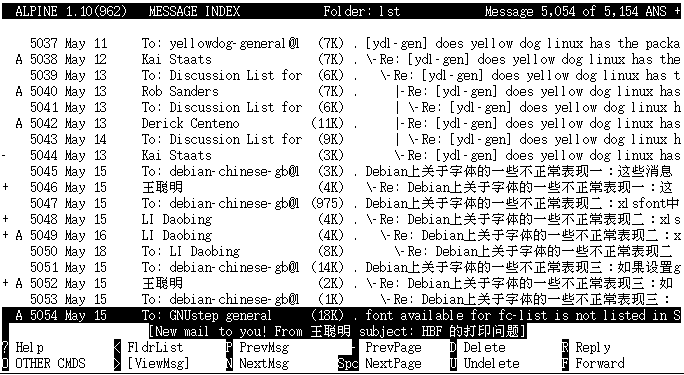
\includegraphics[width=0.7\textwidth]{../images/generalized_parts/03_Alpine_email_client.png}
    \caption{Alpine,一个基于文本用户界面的电子邮件客户端}
    \footnotesize{图片来源:维基共享资源}
\end{figure}
图形用户界面则为用户提供了丰富的输入方式,输出方式也从纯文本扩展到多媒体等各种类型。它在呈现上也更为直观。一个浏览器就是一个典型的图形用户界面程序。笔者还记得自己开始用电脑的时候,很少使用键盘,基本上就是拿着鼠标在点点点。\par
\begin{figure}[htbp]
    \centering
    
\includegraphics[width=0.7\textwidth]{../images/generalized_parts/03_GUI_example_Chrome.png}
    \caption{Chrome,一个典型的图形用户界面程序}
\end{figure}
C++功能丰富,无论是命令行界面还是文本用户界面,我们都可以用代码的方式来实现。而\textbf{本书所介绍的内容全部适用于命令行界面}的编程。我们写出来的程序也全部都是控制台程序(Console Application)。\par
我们与控制台程序的交互往往依靠键盘来实现输入,靠屏幕来实现输出\footnote{并不尽然,比如可以通过文件操作,或者字符串等方式来实现输入、输出。我们会在第十三章和精讲篇中进行解释。}。C++使用\textbf{流(Stream)}来控制输入输出。我在键盘上按下一系列按键,最后按下回车,我的输入信息就以流的方式传递给程序,这是输入;程序得到了我的输入,再经过运算,求得我想要的结果,也以流的方式显示到控制台程序的命令行界面上,这是输出。\par
\subsubsection*{输入}
想像一下我们使用命令行界面时的情形:如图3.3所示,有一个\textbf{光标(Cursor)}在界面上不停闪烁,等待我们输入。当我们按下一个按键,比如 \lstinline@d@,光标的位置上就会出现一个 \lstinline@d@,同时光标后移一位。如果我们按下退格键,光标就会前移一位,并删除上一个输入字符。如果用方向键前移光标的位置并再次输入内容,还可能把之前的输入覆盖掉\footnote{只在覆盖模式下有效。计算机文字处理器都有输入两种模式:插入模式和覆盖模式。对于有些系统来说,命令行界面默认使用的是插入模式。}。\par
\begin{figure}[htbp]
    \centering
    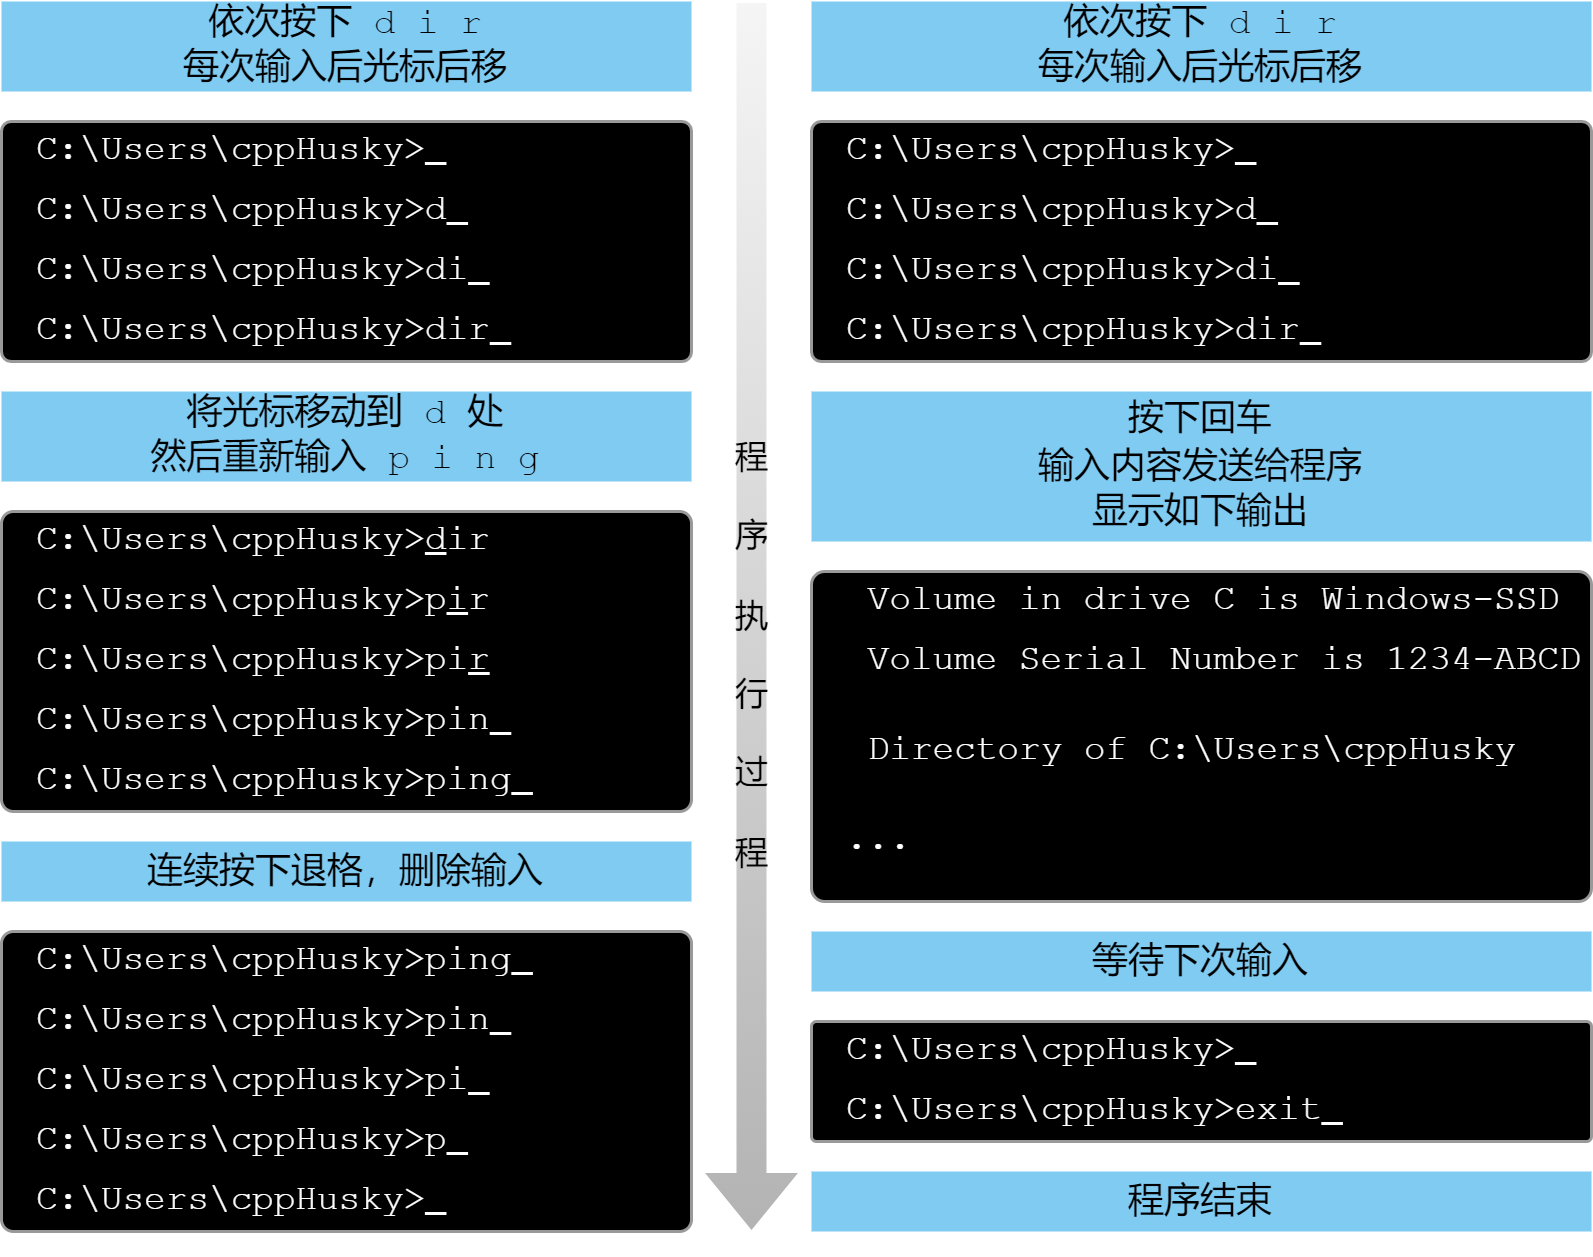
\includegraphics[width=\textwidth]{../images/generalized_parts/03_input_to_cmd_300.png}
    \caption{命令行界面输入场景示例}
\end{figure}
值得注意的是回车键。在我们按下回车键之前,我们输入的内容并未实际发送给计算机,我们可以修改这些内容;而一旦按下了回车键,本行的输入内容将会发送给程序\footnote{这才是真正意义上完成了一次输入。},我们也没机会再修改了。\par
那么当我们按下回车键之后,计算机将会接收到什么输入内容呢?我们可以用这个程序来检测:
\lstinputlisting[caption=\texttt{Input\_to\_ASCII.cpp},label={lst:InputToASCII}]{../code_in_book/3.1/Input_to_ASCII.cpp}\par
读者可以自行尝试这个程序。如果你单独按下一个回车键,程序会给出输出 \lstinline@10@。\textbf{这说明,回车键也是一种输入!}当你按下回车键的时候,既有``发送输入内容''的作用,又有``输入一个回车字符''作用。这点我们现在还不必深究,读者只需有一个印象即可。\par
\subsubsection*{输出}
如果说输入是我们在命令行中敲下若干字符的过程的话,那么输入就是程序在命令行中敲下若干字符的过程。\footnote{这当然是不严谨的。一般来说输出流有缓冲区机制,会先把输出内容存入缓冲区,再一次性将缓冲区内容输出,以提高效率。程序输出的逻辑与人工输入并不相同!这里只为方便初学者理解而如是描述。}想象一下,在输出过程中有一个输出光标,程序每输出一个字符,光标就会后移一位;输出换行符时,程序就会换行。\par
以后我们会谈及更多细节,这里就不再赘述。\par
\subsection*{程序的结构}
科拉多·博姆\footnote{科拉多·博姆(Corrado Böhm),意大利计算机科学家,以其对结构化程序理论和$\!\lambda\!$演算等的贡献而闻名。}和朱塞佩·雅可比尼\footnote{朱塞佩·雅可比尼(Giuseppe Jacopini),意大利数学家和计算机科学家,结构化程序理论的提出者之一。}于1966年在论文\footnote{\textit{Flow Diagrams, Turing Machines And Languages With Only Two Formation Rules},1966年发表于《ACM通讯》。}中提出了\textbf{结构化程序理论(Structured program theorem)}。结构化程序理论证明了,任何计算过程都可以用以下三种结构及其组合来表示:
\begin{itemize}
    \item 一个接一个地执行一系列操作,这叫做\textbf{顺序(Sequence)}。
    \item 根据一个判断条件\footnote{一般是一个 \lstinline@bool@ 变量,或者可以隐式类型转换为 \lstinline@bool@ 类型的数据。当然,\lstinline@switch@ 语句是个例外。},选择执行两个操作中的一个,这叫做\textbf{选择(Selection)}。
    \item 只要满足某个判断条件,就重复执行某个操作,直至条件不满足,这叫做\textbf{循环(Iteration/Loop)}。
\end{itemize}
图3.4是对结构化程序理论的直观解释。\par
\begin{figure}[htbp]
    \centering
    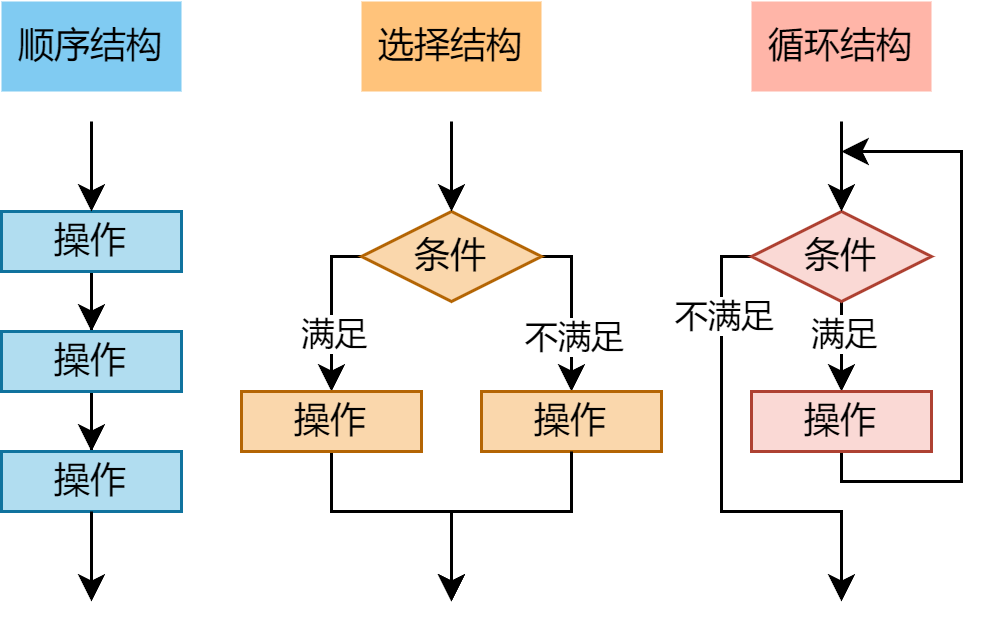
\includegraphics[width=0.6\textwidth]{../images/generalized_parts/03_structured_program_theorem_300.png}
    \caption{顺序、选择和循环结构}
\end{figure}
对于顺序结构,我们已经很熟悉。我们之前已经尝试了好几个程序的代码。在这些程序的主函数中,代码的顺序就对应着程序执行的顺序。所以一个变量要先定义,后使用。
\begin{lstlisting}
    int a {1234}; //先定义
    cout << a; //后使用
\end{lstlisting}
如果把这两句代码的顺序颠倒,编译器就会报错。
\begin{lstlisting}
    cout << a; //先使用
//error: 'a' was not declared in this scope
    int a {1234}; //后定义
\end{lstlisting}
报错信息的意思是,``\lstinline@a@ 尚未定义''。\par
所以说程序运行过程中还有一个不得不关注的次序问题,我们马上就来讲解一些有关的例子。\par
\subsection*{语句的运算次序}
C++中有一对有趣的运算符:自增运算符 \lstinline@++@ 和自减运算符 \lstinline@--@。\par
自增运算符作用于各种类型的变量\footnote{包括整型、浮点型和字符型,乃至指针等类型。但 \lstinline@bool@ 型是个例外,C++17标准起已明文禁止对 \lstinline@bool@ 进行自增和自减运算。},可以使它的值增加 \lstinline@1@。自减运算符反之,可以使它的值减小 \lstinline@1@\footnote{但不要忘记每个类型都有它的范围和精度限制。对 \lstinline@int@ 表示范围的最大值自增将会发生溢出;对 \lstinline@1e50@ 这种过大的数据自增/自减已经超出了其精度承受范围。}。如果我们反复操作自增或自减运算符,可以使数据增加或减小任意值。这种性质使其在循环结构中很好用,我们之后就会介绍。\par
自增运算符的语法有两种,自减运算符的语法可以仿照写出来,我就不赘述了。
\begin{lstlisting}
    <变量> ++; //后缀自增运算
    ++ <变量>; //前缀自增运算
\end{lstlisting}
它们实现的功能都是为 \lstinline@<变量>@ 加一,但区别在于``返回值''。前缀自增的返回值是增加之后的值;而后缀自增的返回值是增加之前的值。让我们用一个很简单的例子来说明这个问题吧:
\begin{lstlisting}
    int a {3}; //定义a=3
    cout << a++ << ' '; //输出a++,观察返回值
    cout << a << endl; //输出a,观察a的值
    cout << ++a << ' '; //输出++a,观察返回值
    cout << a;         //输出a,观察a的值
\end{lstlisting}
程序的运行结果如下:\\\noindent\rule{\linewidth}{0.2pt}\texttt{
3 4\\
5 5
}\\\noindent\rule{\linewidth}{0.2pt}\par
程序给了两行输出,第一行分别是 \lstinline@a++@ 的返回值和 \lstinline@a@ 的值。可以看出,\lstinline@a@ 在自增之后给到的返回值依然是原来的(增加之前) \lstinline@3@;而这时 \lstinline@a@ 的值其实是 \lstinline@4@。第二行分别是 \lstinline@++a@ 的返回值和 \lstinline@a@ 的值。可以看出,\lstinline@a@ 在自增之后给到的返回值就是增加之后的值了。\par
自减运算符的道理是相同的,读者可以把上述代码中的 \lstinline@++@ 全部改成 \lstinline@--@,先猜一下它的运行结果,然后再编译运行一下,检验你的猜想。不出意外的话,程序的运行结果应当是:\\\noindent\rule{\linewidth}{0.2pt}\texttt{
3 2\\
1 1
}\\\noindent\rule{\linewidth}{0.2pt}\par
一些人会把前缀自增/自减和后缀自增/自减的区别解释为``前缀写法是先加后用,后缀写法是先用后加''。这种理解方式很直观,先加后用就是先增加,再提供返回值;先用后加就是先提供返回值,再增加。\par
但是我在这里也要提醒读者,这种理解方式未必是正确的!对于内置类型的自增/自减运算来说,不同编译器可能给出不同的运算方式。如果读者能够理解汇编\footnote{汇编语言(Assembly language),是一类用于各种可编程器件的低级语言。汇编语言不是一个单一的语言,它是一系列语言的统称。汇编语言的指令集严重依赖于具体的器件,不同的器件可能采用不同的指令集,因而汇编代码的可移植性很差。}代码,可以比较一下x86 msvc v19.38和x86-64 gcc 13.2如何编译这段代码:
\begin{lstlisting}
    int a {3}, b {a ++};
\end{lstlisting}
答案是,x86 msvc v19.38将后缀自增处理为``先用后加'',先返回这个变量本身,再进行自增运算;而x86-64 gcc 13.2将后缀自增处理为``先加后用'',先进行自增运算,再提供返回值,而且此处的返回值不是这个变量本身,而是一个存储了原先值的临时变量。\par
\begin{figure}[htbp]
    \centering
    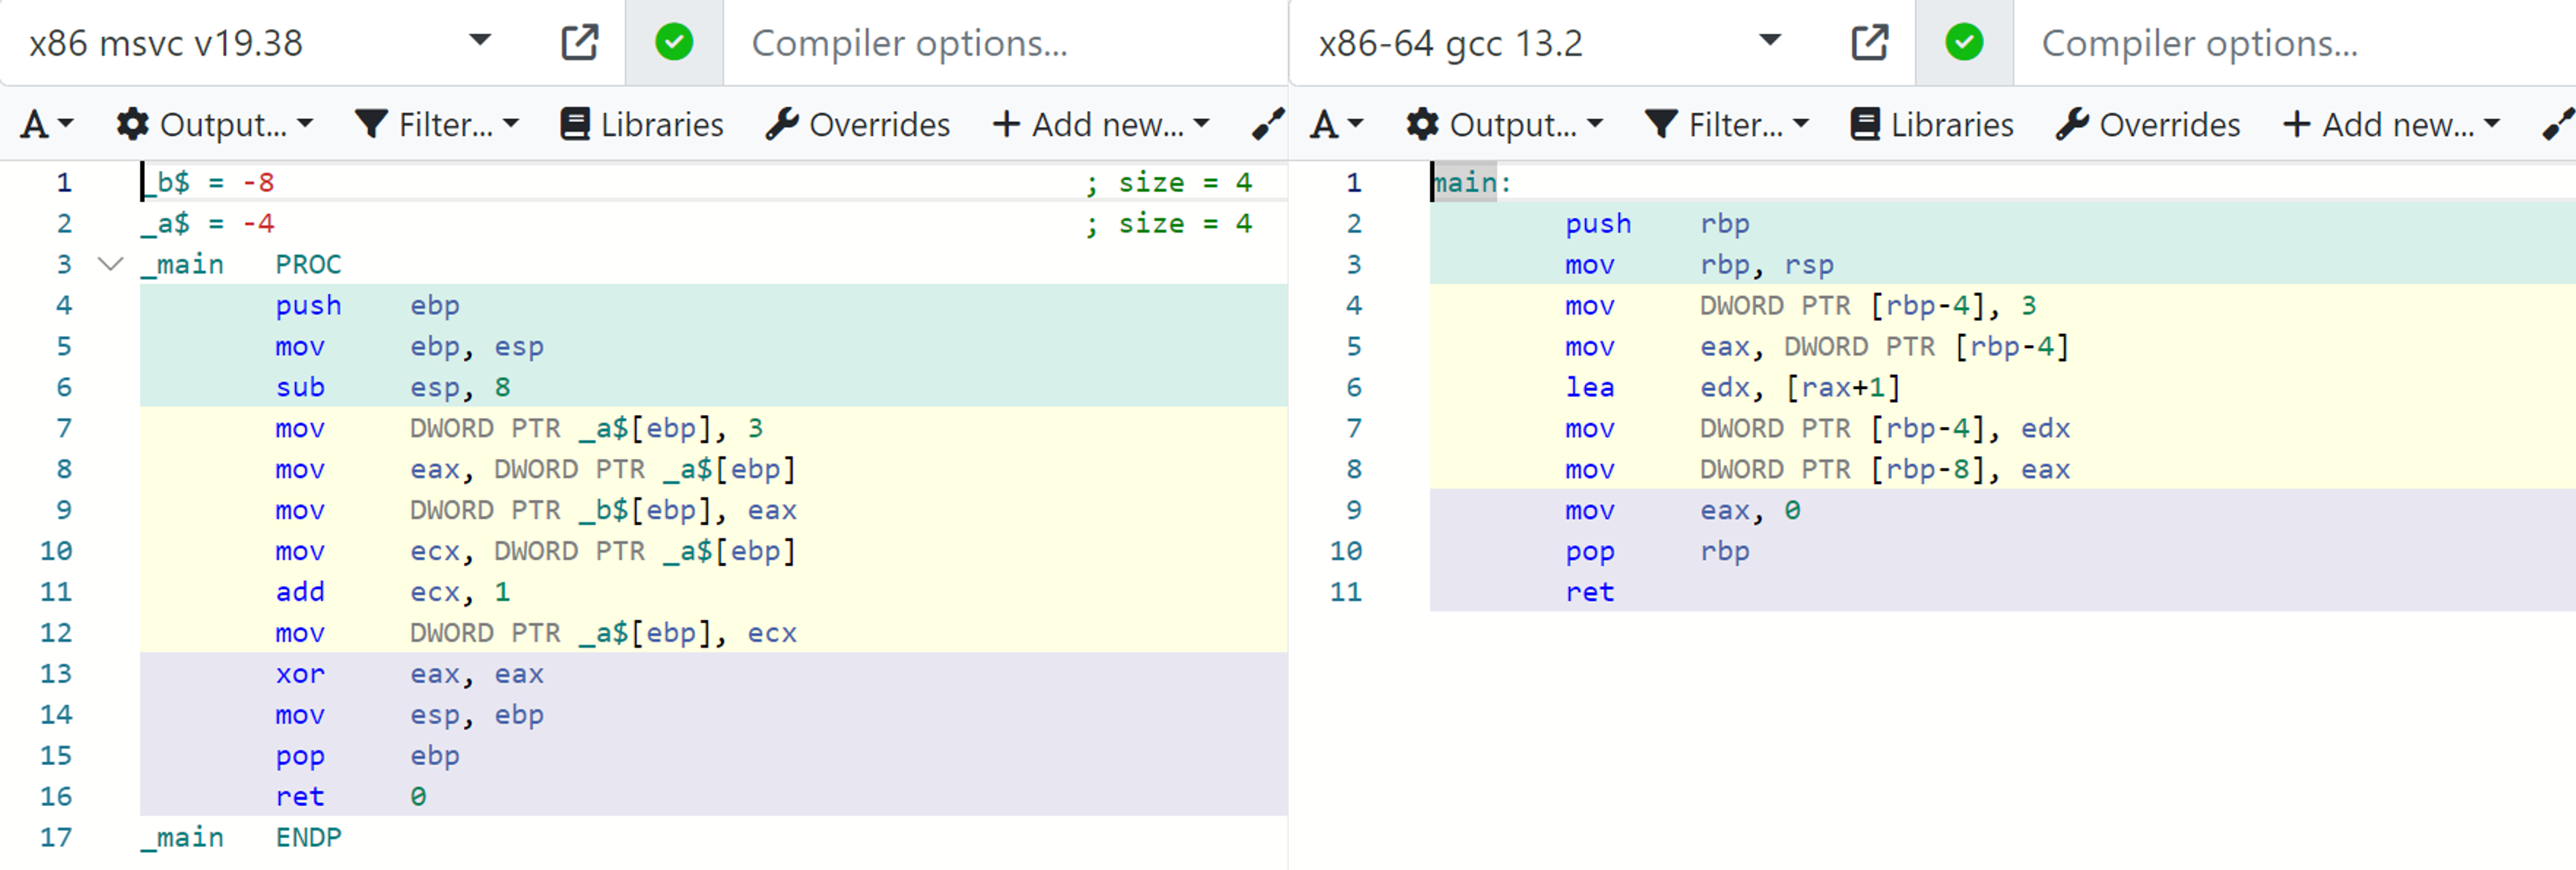
\includegraphics[width=\textwidth]{../images/generalized_parts/03_how_compilers_interpret_postfix_increment.png}
    \caption{后缀自增运算在不同编译器下的汇编代码}
    \footnotesize{左图为x86 msvc v19.38;右图为x86-64 gcc 13.2\\编译支持:\href{https://godbolt.org/}{Compiler Explorer}}
\end{figure}
读者尚无必要去纠结这些细节,只需从这个例子中体会到,很多时候,我们或别人``总结''出来的规律只是一种管中窥豹,仅在一定范围内是正确的;一旦离开这个范围,这些规律非但可能不适用,还有可能会为我们准确理解事物逻辑造成更大的障碍。所以读者必须具备这样的意识,对于各种第三方——包括本书在内——总结出来的``规律''保持警觉,并最好通过亲手操作的方式来验证之。\par
回到自增/自减运算。考虑这样一个赋值语句:\lstinline@b=a++@。自增/自减运算符的优先级比赋值运算符的优先级高,所以它可以解释为 \lstinline@b=(a++)@。我们可以进一步把这个过程拆解成三个操作:赋值,\lstinline@a@ 增加一,以及 \lstinline@a++@ 提供返回值。那么问题来了,哪个操作在先,哪个操作在后呢?这就是\textbf{次序(Order)}问题了。\par
首先我们不难理解,``\lstinline@a++@ 提供返回值''这个操作肯定要早于``赋值''操作。否则赋值语句就不知道该赋什么值。既然要算出返回值,那么赋值运算符右边的所有操作都应该在赋值之前做完,于是``\lstinline@a@ 增加一''这个操作肯定也早于``赋值''操作。\par
接下来问题来了,``\lstinline@a@ 增加一''和``\lstinline@a++@ 提供返回值''这两个操作谁先谁后呢?刚才我们就看到了,\textbf{不同编译器会给出不同的操作次序}。但是无论以何种次序以何种次序计算,编译器总会给出正确的结果。\footnote{我们也称之为``不定序''。一般来说,这种不定序的情况不会影响到我们的日常编程,因为结果总是一样的。但是也请注意防范``未定义行为''的发生,我们会在后面讲到。}\par
但是并非所有这类操作都能给出``正确的结果''——或者说,压根就没有正确的结果!一个最经典的例子就是
\begin{lstlisting}
    int a {0};
    cout << a++ + a++;
\end{lstlisting}
这段代码在不同编译器下的结果是不同的,而且也没有标准答案!其原因在于,加法运算符并不确定左右各个操作的顺序。\par
如果要追究本源,这就要看C++标准是如何规定的了。C++17起的标准明确规定,\lstinline@=@ 右端的所有值计算和副作用发生\footnote{值计算和副作用将在第四章讲解。在此之前我们可以把它们当作所有操作的统称。}都要早于左端的任何值计算和副作用发生。而C++标准仍未规定加法运算符两端操作的运算次序,所以不同编译器就有不同的理解。\par
\subsubsection*{逻辑运算符}
在C++标准中,有三个逻辑运算符:逻辑非(\lstinline@!@)、逻辑与(\lstinline@&&@)和逻辑或(\lstinline@||@)。它们在选择和循环结构中很常用,所以在这里不得不提。我们在前面已经分析了很多运算符,这里只要按照相同的思路来分析就可以了。先来分析逻辑与运算符。\par
\begin{figure}[htbp]
    \centering
    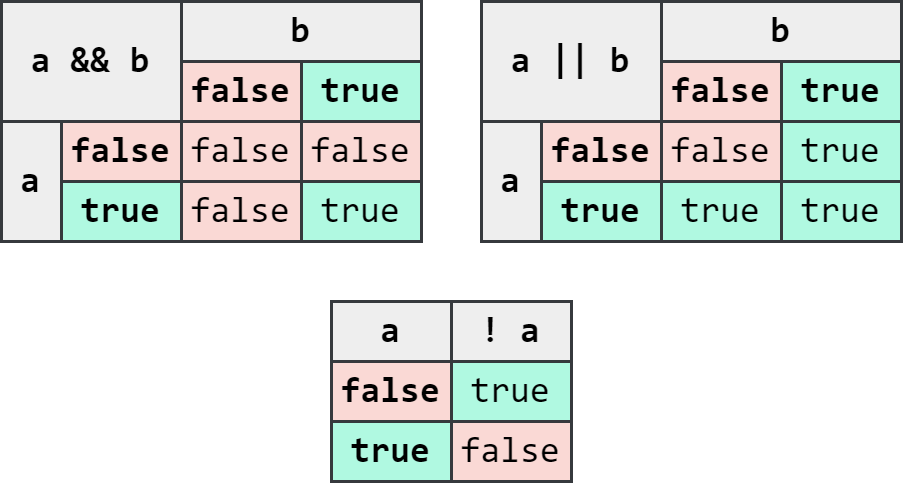
\includegraphics[width=0.8\textwidth]{../images/generalized_parts/03_truth_table_of_logic_operators_300.png}
    \caption{逻辑与、逻辑或、逻辑非运算符的真值表}
\end{figure}
逻辑与运算符只能接收 \lstinline@bool@ 类型的操作数;非 \lstinline@bool@ 型的操作数都会通过\hyperref[con:boolean_conversions]{布尔转换}来变成 \lstinline@bool@ 型。\par
逻辑与运算符的返回值也是 \lstinline@bool@ 类型,只有当两个操作数的值都为 \lstinline@true@ 时,它的返回值才是 \lstinline@true@,否则就是 \lstinline@false@。\par
逻辑或运算符和逻辑与运算符很相像,唯一的区别是返回值,只有当两个操作数的值都为 \lstinline@false@ 时,它的返回值才是 \lstinline@false@,否则就是 \lstinline@true@。\par
简单说来,逻辑与运算符要求两个操作数都为真,而逻辑或运算符要求两个操作数有至少一个为真\footnote{在不同语境下,自然语言中的``或''可能指的是``互斥或''或者``可兼或''。而编程语言中的``异或''与``或''是有很明确的规则的,不可混淆。}。\par
逻辑非运算符比较特殊,它只有一个操作数\footnote{像逻辑非、自增/自减运算符这种仅有一个操作数的运算符,我们有时称它们为一元运算符或单目运算符。},而且只能以前缀的形式表达。\lstinline@!a@ 是正确的,但 \lstinline@a!@ 就不对了。\par
逻辑非的功能不复杂:如果操作数的值是 \lstinline@true@,返回值就是 \lstinline@false@;如果操作数的值是 \lstinline@false@,返回值就是 \lstinline@true@。但是要注意:\textbf{逻辑非运算符不能直接改变操作数的值},这和自增/自减运算符是不一样的。比如 \lstinline@!a@,完了之后 \lstinline@a@ 的值是不变的。\par
关于这三个运算符的优先级和结合性,读者可以自行查阅附录A的表,我这里就不谈了。图3.6是这三个运算符的真值表,读者可以对照此表,加深对这三种运算符的印象。\par
至于运算次序,C++对于逻辑与/逻辑或运算符的运算次序有明文规定,运算符左边的操作必须早于右边的操作完成。\par
\subsubsection*{短路求值}
逻辑与/逻辑或运算符有一个\textbf{短路求值(Short-circuit evaluation)}的特性。对于 \lstinline@&&@ 运算符来说,如果左操作数的值算完了,发现是 \lstinline@false@,那么无论右操作数的值是什么,整个表达式的返回值都只可能是 \lstinline@false@ 了。于是程序为了节省时间,就会跳过右操作数的计算。
\begin{lstlisting}
    constexpr int init {0}; //定义常量表达式init,值为1
    int a {init}; //用init来初始化变量a
    a++ && a++; //用&&连接两个a++,预期会使a自增两次
    cout << a - init; //a当前值减去初始值,预期输出2
\end{lstlisting}
这个程序的最终输出为:\texttt{1}。这可能有点令人吃惊,但仔细分析一下,你就会明白其中原因了。\par
在 \lstinline@a++ && a++@ 语句中,\lstinline@&&@ 的左操作数会优先计算(C++标准明文规定),这里 \lstinline@a++@ 后缀自增,使 \lstinline@a@ 变为 \lstinline@1@,而返回值为 \lstinline@0@。\par
根据布尔转换规则,\lstinline@0@ 将转换为 \lstinline@false@,这说明无论右操作数为何,整个计算的结果必然是 \lstinline@0@,于是右操作数的计算过程被跳过,到输出的时候,\lstinline@a@ 还是 \lstinline@1@,减去 \lstinline@init@ 当然就是最终结果 \lstinline@1@ 了。\par
读者可以把 \lstinline@init@ 改为 \lstinline@1@ 或者是其它数,输出结果将变为 \lstinline@2@。\par
关于 \lstinline@||@ 的短路求值是同理的,如果左操作数的值是 \lstinline@true@,就会跳过右操作数的计算过程。这不是本章的重点,所以我就不再赘述了。\par
